\documentclass{sigchi-ext}
% Please be sure that you have the dependencies (i.e., additional
% LaTeX packages) to compile this example.
\usepackage[T1]{fontenc}
\usepackage{textcomp}
\usepackage[scaled=.92]{helvet} % for proper fonts
\usepackage{graphicx} % for EPS use the graphics package instead
\usepackage{balance}  % for useful for balancing the last columns
\usepackage{booktabs} % for pretty table rules
\usepackage{ccicons}  % for Creative Commons citation icons
\usepackage{ragged2e} % for tighter hyphenation

% Some optional stuff you might like/need.
% \usepackage{marginnote} 
% \usepackage[shortlabels]{enumitem}
% \usepackage{paralist}
% \usepackage[utf8]{inputenc} % for a UTF8 editor only

%% EXAMPLE BEGIN -- HOW TO OVERRIDE THE DEFAULT COPYRIGHT STRIP --
\copyrightinfo{Submitted to UbiComp/ISWC 2018}

%Permission to make digital or hard copies of all or
% part of this work for personal or classroom use is granted without
% fee provided that copies are not made or distributed for profit or
% commercial advantage and that copies bear this notice and the full
% citation on the first page. Copyrights for components of this work
% owned by others than ACM must be honored. Abstracting with credit is
% permitted. To copy otherwise, or republish, to post on servers or to
% redistribute to lists, requires prior specific permission and/or a
% fee. Request permissions from permissions@acm.org.\\
% {\emph{CHI'14}}, April 26--May 1, 2014, Toronto, Canada. \\
% Copyright \copyright~2014 ACM ISBN/14/04...\$15.00. \\
% DOI string from ACM form confirmation}
%% EXAMPLE END

% Paper metadata (use plain text, for PDF inclusion and later
% re-using, if desired).  Use \emtpyauthor when submitting for review
% so you remain anonymous.
\def\plaintitle{EyeWear 2018: Second Workshop on EyeWear Computing} \def\plainauthor{First Author, Second Author, Third Author,
  Fourth Author}
\def\emptyauthor{}
\def\plainkeywords{Eyewear, Head-mounted Displays, Smart Glasses, Virtual Reality, Augmented Reality, Activity Recognition, Perception-Aware Computing,
Human Augmentation}
\def\plaingeneralterms{Documentation, Standardization}

\title{\plaintitle}

\numberofauthors{7}
\author{%
  \alignauthor{
  \textbf{Benjamin Tag}\\
    \affaddr{Keio University}\\
    \affaddr{Yokohama, Japan}\\
    \email{tagbenja@kmd.keio.ac.jp}}
  \alignauthor{%
  \textbf{Olivier Augereau}\\
    \affaddr{Osaka Prefecture University}\\
    \affaddr{Osaka, Japan}\\
    \email{augereau.o@gmail.com}}\vfil 
  \alignauthor{
 \textbf{Christian Holz}\\
    \affaddr{Microsoft Research}\\
    \affaddr{Redmond, US}\\
    \email{cholz@microsoft.com}
    }
  \alignauthor{ 
  \textbf{Yuji Uema}\\
    \affaddr{J!NS Inc.}\\
    \affaddr{Tokyo, Japan}\\
    \email{yuji-uema@jin-co.com}
 }\vfil
  \alignauthor{
  \textbf{Paul Lukowicz}\\
    \affaddr{DFKI}\\
    \affaddr{Kaiserslautern, Germany}\\
    \email{paul.lukowicz@dfki.de}}      
  \alignauthor{
  \textbf{Kai Kunze}\\
    \affaddr{Keio University}\\
    \affaddr{Yokohama, Japan}\\
    \email{kai.kunze@gmail.com}
    }\vfil
}




% Make sure hyperref comes last of your loaded packages, to give it a
% fighting chance of not being over-written, since its job is to
% redefine many LaTeX commands.
\definecolor{linkColor}{RGB}{6,125,233}
\hypersetup{%
  pdftitle={\plaintitle},
%  pdfauthor={\plainauthor},
  pdfauthor={\emptyauthor},
  pdfkeywords={\plainkeywords},
  bookmarksnumbered,
  pdfstartview={FitH},
  colorlinks,
  citecolor=black,
  filecolor=black,
  linkcolor=black,
  urlcolor=linkColor,
  breaklinks=true,
}

% \reversemarginpar%

\begin{document}

\maketitle
% Uncomment to disable hyphenation (not recommended)
% https://twitter.com/anjirokhan/status/546046683331973120
\RaggedRight{} 
% Do not change the page size or page settings.
\begin{abstract}
Virtual/augmented reality headsets, smart sensing glasses and  and similar "smart eyewear" have recently emerged as commercial products and can provide an interesting research platform for a range of research fields, including human-computer interaction, ubiquitous computing, pervasive sensing, and social sciences. The proposed workshop will bring together researchers from a wide range of computing disciplines, such as mobile and ubiquitous computing, eye tracking, optics, computer vision, human vision and perception, usability, as well as systems research. The workshop is a continuation from a 2016 and will focus on discussing application scenarios and shared interest use cases for eyewear computing between corporate and academic researchers. 
\end{abstract}
\keywords{\plainkeywords}

\category{H.5.m}{Information interfaces and presentation (e.g., HCI)}{Miscellaneous}



\section{Introduction}
We often believe the face to be a reflection of our personality or character. It holds most of our senses - sight, hearing, taste, smell and is used to express affect. Head and face seem to be an obvious choice to place sensors and actuators to track user's activities and provide interaction possibilities~\cite{amft2015making,kuhn2016gphysics}. 
\begin{marginfigure}[0pc]
 \begin{minipage}{\marginparwidth}
   \centering  
      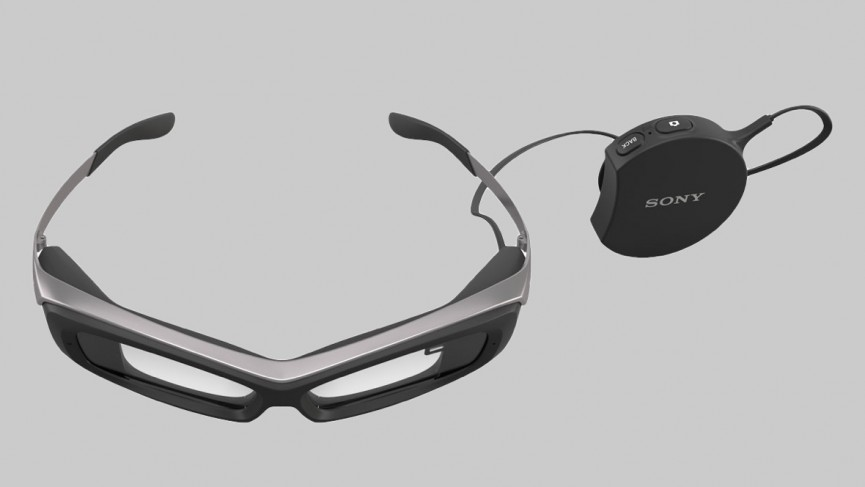
\includegraphics[width=\columnwidth]{figures/sony.jpg}
         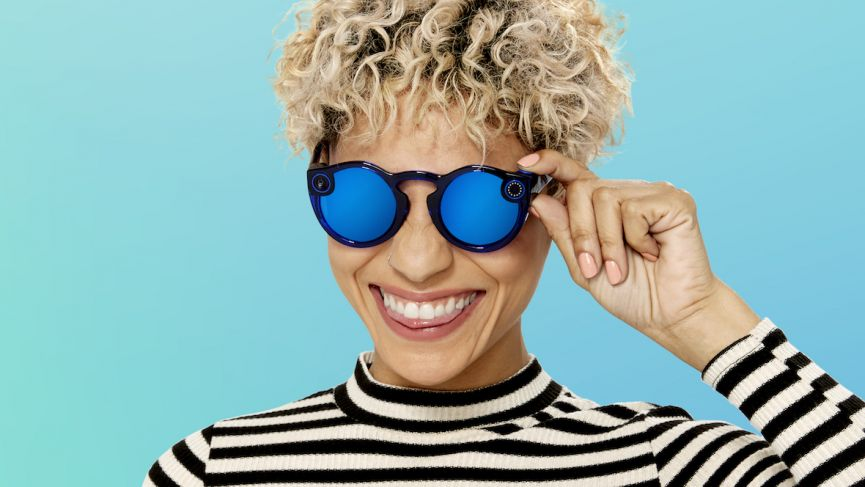
\includegraphics[width=\columnwidth]{figures/spectales.jpg}
           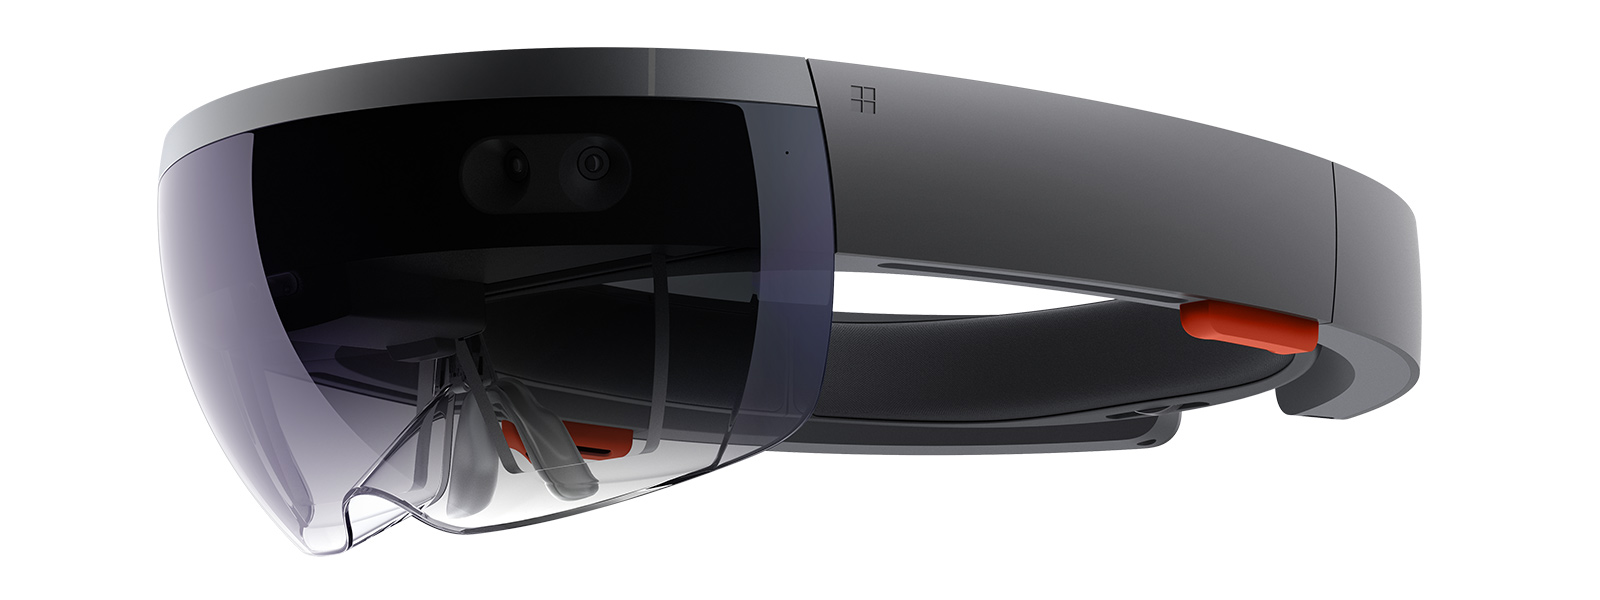
\includegraphics[width=\columnwidth]{figures/holo.jpg}
   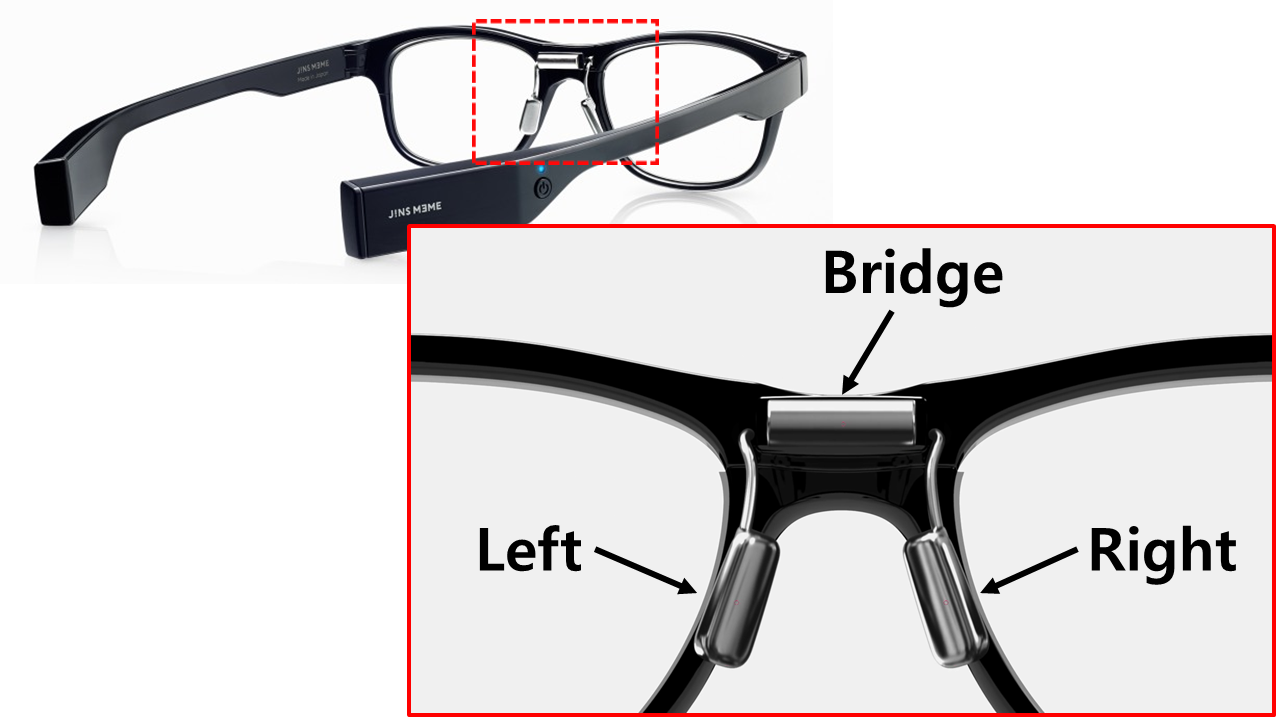
\includegraphics[width=\columnwidth]{figures/1-4}

  \caption{Examples of commercial smart eyewear. Sony Smart glasses, Snapchat Spectacles, Microsoft Hololense, J!NS MEME.}~\label{fig:glasses}
 \end{minipage}
\end{marginfigure} However, for a long time, head/face based wearables have been restricted to special purpose, niche applications.  While hearing aids and mobile headsets are widely accepted as head-worn devices, users in public spaces often consider novel head-attached sensors and devices as uncomfortable, irritating, or stigmatizing. Yet, given a number of recent technological, we believe eyewear computing will soon transition into mainstream technology and prominent research field. In essence, because the face is so important to humans, under every day circumstances people are highly sensitive to ergonomic and social acceptance aspects of anything placed there. It is telling that in early wearable computing ergonomic studies the head was not even included~\cite{bodine2003effects}. Early ego-centric vision devices were rather bulky, expensive, and their battery lifetime severely limited their use to short durations of time\cite{cakmakci2006head}. Building on existing work in wearable computing, recent commercial egocentric vision devices and mobile eye trackers, such as Google Glass, SMI ETG, and J!NS meme, pave the way for a new generation of "smart eyewear" that are light-weight, low-power, convenient to use, and increasingly look like ordinary glasses\cite{bulling2014cognition,kliegl2006tracking}.

This workshop proposal is motivated by the observation that, through a combination of consumer attitude shifts and technological advances, complex head/face based sensing/interaction is increasing becoming feasible for use in every day real world situations. We've seen in recent years that Eyewear Computing transitioned from a mere academic research interest to commercially viable products (see Figure~\ref{fig:glasses}). Recent advances in real-life tracking of physical and cognitive activities (e.g. reading, detection of fatique, concentration) are additional enabling technologies for new application fields towards a quantified self for the mind~\cite{kunze2015quantifying}.
The workshop is a continuation of the first EyeWear 2016 at UbiComp Heidelberg, which focused mostly on the enabling technologies. We will still discuss enabling sensors and actuators, yet in contrast to 2016, we will focus more on application scenarios and creating the academic and corporate connections for an open eyewear platform to foster exchanges in sensing, interaction, hardware and software know-how.

\section{Topics}

As Smart Eyewear can be a powerful enabling technology for a broad range of research fields, we plan to tackle the following topics during the seminar with a special focus on forming a community to exchange hardware designs, requirements, best practices and source code to build and run Smart Eyewear prototypes. The areas of interest include:

 {\bf Novel application cases:} Which activities are the most useful for application cases that have the most impact on society. What are the best application fields to apply smart eyewear for the strongest impact on society?
 
{\bf Suitable Sensing and actuation technologies:} Driven by the application cases which sensing modalities are the most interesting to be integrated in smart eyewear? What are the important activities to focus on (e.g. fatigue detection, concentration tracking)? 

 {\bf Impact and perils of long-term sensing:} How can we use these real life recordings of physical, physiological and cognitive signals on the head? What are potential negative effects of long term usage, ranging from perceptual issues regarding the use of wearable displays (binocular rivalry, vertical and horizontal gaze comfort, instrument myopia, eye strain, accommodation-convergence mismatch) to potential skin irritations during the deployment of electrodes, or other sensors necessary to touch the skin. 

{\bf Towards an Open Eyewear Platform:} How can we build up an international community to share scientific results and work together on topics related to Smart Eyewear. Especially when we discuss large scale, long monitoring of cognitive activities, we believe a strong impact on psychology, sociology and cognitive science as eyewear computing can be an enabling technology for them to  become less model and more data driven sciences utilizing real world setups instead of controlled but artificial laboratory settings.

\section{ACTIVITIES}
We propose a one-day workshop {\bf on the 8th October} with presentation sessions in the morning, development of scenarios in the early afternoon, and group discussions on fundamental challenges in the late afternoon. In the following we describe pre-workshop preparations and the post-workshop follow up.

\subsection{Presentations}
The workshop will start with an introduction and the keynote to the workshop topic (10:00-12:30), followed by short introductory presentations to get familiar with the participants and the topics they are working on. 
Keynotes will be given by Prof. Thad Starner and Ozan Cakmakci (both  tentatively confirmed). Ozan Cakmakci is a lead optical research and development engineer focusing on future optical architectures for Google Glass at Google[x]. Prof. Starner is the director of the Contextual Computing Group (CCG) and is also the longest-serving Technical Lead/Manager on Google Glass. 
Authors will get 5 minutes to present their work keeping presentations short and focused. While listening to the presentations, all participants will be asked to take notes on provided Post-Its, which we will share on a large whiteboard in order to prepare for the discussion sessions.
The presentation session will be broken into two parts with a short coffee break in between. This will allow enough time to discuss different ideas coming out from the presentations.

\subsection{Demonstration Session}
We encourage participants to bring and show demonstrations of research prototypes related to their submissions. Depending on the number of demonstrations we will hold a separate demonstration session or do small show-and-tells in the coffee breaks.

\subsection{Scenario Development}
After the presentation sessions, workshop participants will start developing scenarios in groups. All participants will write notes on Post-Its, which will be added to the Post- Its from the morning session on the whiteboard. In order to sort out the challenges and opportunities for technologies that augment the human mind, we will create an affinity diagram analysis of the Post-Its. Group analysis will start at 15:00 and will end at 15:30.

\subsection{Group Discussion}
After the group analysis we will have a longer coffee break (15:30-16:00) and then discuss identified challenges and opportunities (16:00-17:00). The organizers will actively inter- act with the audience to stimulate discussion. After that we will summarize key experiences from the workshop and will plan follow up activities (17:00-17:30).

\subsection{Post-Workshop Follow Up}
At the workshop organizers will take pictures/document the outcome of the analysis and the content on the whiteboard. This will be made available to the workshop participants through a shared Google Drive folder. The participants will be invited to an existing Slack Channel where they can share relevant papers to the workshop themes.

\section{Organizers}

{\bf Benjamin Tag} is a researcher at Keio Media Design working on smart eyewear research topics focusing on fatigue detection in real life situations and on creating feedback loops for responsive media using head worn sensing.

{\bf Oliver Augereau} is an Research Assistant Professor at Osaka Prefecture University in the intelligent media processing group which is supervised by Professor Koichi Kise. He use devices such as cameras, eye-trackers, and smart glasses in order to get information from the reading activity. He researches also "experiential supplements". The aim is to create new tool for sharing experiences for improving learning and education.

{\bf Christian Holz} is a researcher at Microsoft Research, Redmond, WA, focusing on novel human-computer interfaces, small and wearable devices, sensing systems, and signal processing.

{\bf Paul Lukowicz} is Full Professor of AI at the Technical University of Kaiserslautern in Germany where he will head the Embedded Intelligence group at DFKI. His research focus is context aware ubiquitous and wearable systems including sensing, pattern recognition, system architectures, models of large scale self-organized systems, and applications.

{\bf Kai Kunze} works as an associate project professor at Keio Media Design, Keio University. Beforehand, he held an assistant professorship at Osaka Prefecture University.  His major research contributions are in pervasive computing, especially in sensing, physical and cognitive activity recognition. Recently, he focuses on tracking knowledge acquisition activities, especially reading.


%\section{Acknowledgements}
%This workshop is based on a Dagstuhl Seminar on EyeWear Computing No. 16042 http://www.dagstuhl.de/16042 . We want to thank the Dagstuhl Team for providing a stimulating environment for research discussions. 

\balance{} 

\bibliographystyle{SIGCHI-Reference-Format}
\bibliography{sample}

\end{document}

%%% Local Variables:
%%% mode: latex
%%% TeX-master: t
%%% End:
